\section{Introducción}

\subsection{Antecedentes y Motivación}

Aunque los sistemas satelitales han evolucionado notablemente en las últimas décadas, pocos avances han impactado tanto su arquitectura como la llegada de los satélites definidos por software. La posibilidad de reconfigurar funciones completas de radio y procesamiento de payloads mediante actualizaciones remotas representa un cambio paradigmático respecto a los diseños basados en hardware dedicado. 

Jiang et al. \cite{Jiang2023} documentan exhaustivamente esta transición hacia redes satelitales definidas por software, destacando cómo la flexibilidad inherente permite adaptar misiones en vuelo, optimizar el uso del espectro y extender la vida útil de las plataformas. Los beneficios resultan evidentes: reducción de costos de desarrollo, mayor capacidad de respuesta ante fallos y la posibilidad de implementar nuevos servicios sin necesidad de reemplazar hardware orbital. No obstante, esta flexibilidad sigue siendo mayoritariamente estática. La mayoría de los SDS actuales dependen de configuraciones predefinidas que, aunque actualizables, carecen de la capacidad de adaptarse de forma autónoma a condiciones cambiantes del entorno espacial.

Resulta revelador observar cómo la convergencia entre software definido y procesamiento de señales digitales abre un terreno fértil para innovaciones más profundas. Uno de los desafíos persistentes radica en dotar a estos sistemas de verdadera inteligencia cognitiva que les permita tomar decisiones en tiempo real ante interferencias, variaciones del canal o cambios en los requisitos de misión.

\begin{figure}[h]
\centering
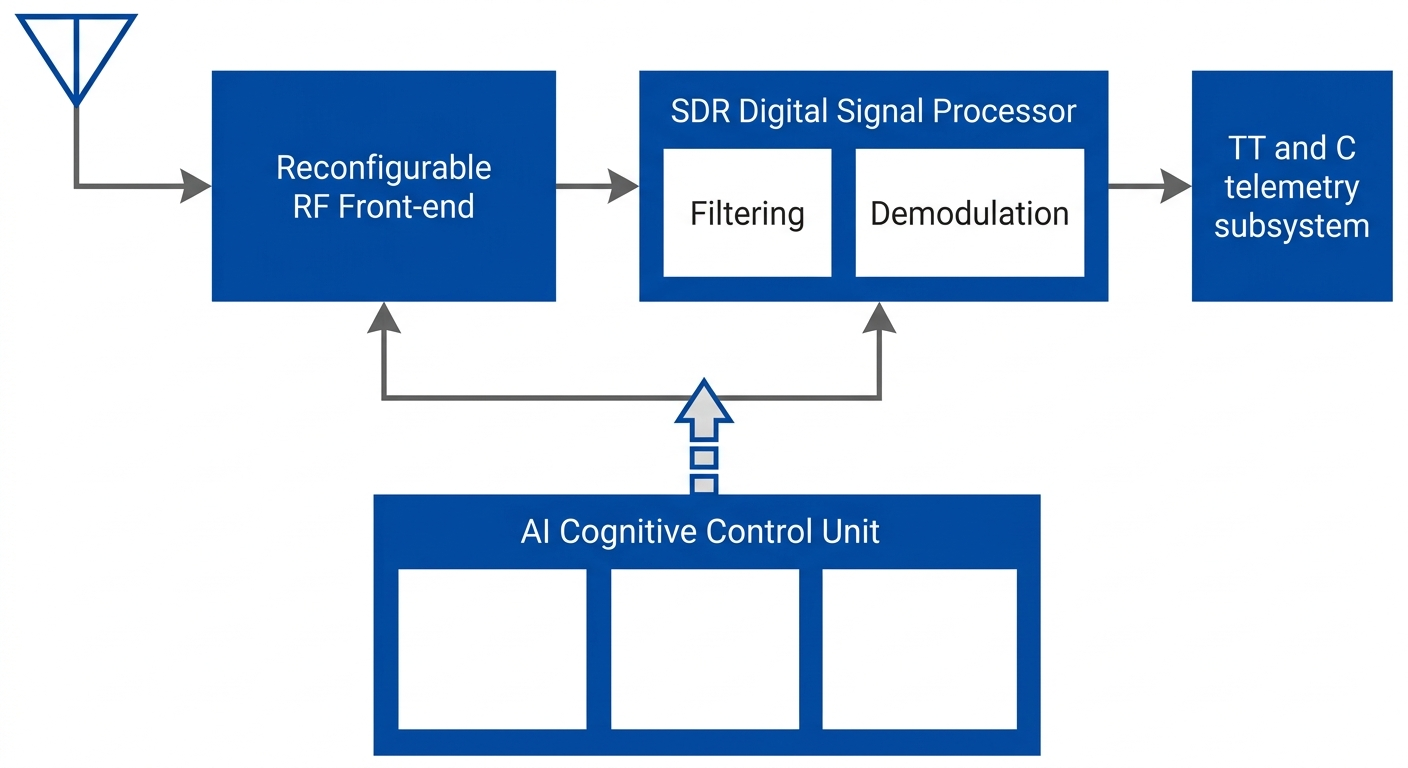
\includegraphics[width=\linewidth]{fig1.png}
\caption{Arquitectura genérica de un satélite definido por software (SDS) mostrando los principales bloques reconfigurables.}
\label{fig:arquitectura_sds}
\end{figure}

\subsection{Problemática Actual}

Lejos de ser un asunto resuelto, la literatura reciente sugiere que los enfoques tradicionales de procesamiento de señales en plataformas SDR presentan limitaciones significativas cuando se enfrentan a escenarios satelitales reales. Aunque los radios definidos por software han mejorado la reprogramabilidad, tienden a operar bajo reglas fijas que resultan insuficientes ante la creciente congestión espectral, la proliferación de constelaciones LEO y la aparición de amenazas dinámicas.

Particularmente llamativo es el hecho de que, en muchos casos estudiados, los sistemas SDR convencionales exhiben un rendimiento aceptable bajo condiciones controladas pero degradan notablemente frente a interferencias no estacionarias o variaciones rápidas del canal espacial. Doha et al. \cite{Doha2026} subrayan en su revisión cómo la integración de técnicas de inteligencia artificial representa el paso natural hacia radios cognitivos capaces de percibir, aprender y actuar de manera autónoma. Sin embargo, la mayoría de implementaciones actuales permanecen en entornos terrestres o simulados, dejando un vacío importante en aplicaciones orbitales donde las restricciones de potencia, latencia y fiabilidad resultan críticas.

\subsection{Contribuciones Principales}

Este trabajo busca precisamente cerrar esa brecha. Se propone un framework de inteligencia artificial especializado en el procesamiento de señales para satélites definidos por software, orientado a incrementar de forma sustancial su flexibilidad operativa y capacidad de adaptación en tiempo real.

Entre las contribuciones principales destacan: el diseño de una arquitectura cognitiva modular que integra modelos de aprendizaje profundo optimizados para entornos con recursos limitados; la aplicación de estas técnicas a tareas críticas como clasificación automática de modulación, estimación de parámetros de señal y mitigación inteligente de interferencias; y la validación exhaustiva utilizando datasets satelitales reales. En este sentido, el conjunto de datos RML24 \cite{Zhang2026}, generado específicamente con plataformas SDR para señales TT\&C, constituye un recurso clave que permite evaluar el desempeño bajo condiciones representativas del canal espacial.

\begin{table*}[h]
\centering
\caption{Comparación entre enfoques SDR y sistemas basados en hardware tradicional}
\label{tab:comparacion_sdr}
\begin{tabular}{lcc}
\hline
\textbf{Característica} & \textbf{Hardware Tradicional} & \textbf{SDR} \\
\hline
Flexibilidad de reconfiguración & Baja & Alta \\
Costo de modificación en órbita & Muy alto & Bajo \\
Tiempo de adaptación a nuevas misiones & Meses & Días/Horas \\
Capacidad cognitiva base & Nula & Limitada \\
Consumo energético típico & Alto & Variable \\
\hline
\end{tabular}
\end{table*}

El resto del artículo se organiza de la siguiente manera. La Sección 2 revisa los antecedentes técnicos y el estado del arte. La Sección 3 detalla la arquitectura propuesta, mientras que la Sección 4 describe la metodología y los experimentos realizados. Los resultados se presentan en la Sección 5, seguidos de su análisis crítico en la Sección 6. Finalmente, la Sección 7 recoge las conclusiones principales y líneas de trabajo futuro.